\documentclass [a4paper] {article}

\usepackage[spanish]{babel} 
\usepackage[utf8]{inputenc} 
\usepackage{multirow} 
\usepackage{float} 

\title{R-PL3}
\author{Gabriel López, Sergio Sanz, Álvaro Zamorano}

\usepackage{Sweave}
\begin{document}

\maketitle

\graphicspath{ {./tmp/} }

\section{Ejercicio realizado en clase.}
Para obtener la \textbf{función de clasificación} mediante el algoritmo construcción
de \textbf{árboles de decisión de Hunt} es necesario usar los paquetes \texttt{rpart} y
\texttt{tree}. Estos paquetes hay que descargarlos desde la página de CRAN y para instalarlos
hay que ejecutar el siguiente código:

\begin{Schunk}
\begin{Sinput}
> install.packages("./Paquetes/rpart_4.1-15.zip")
> install.packages("./Paquetes/tree_1.0-40.zip")
\end{Sinput}
\end{Schunk}

\bigskip
De esta forma, los paquete únicamente estarán instalados. Para poder usarlos es necesario cargarlos:
\begin{Schunk}
\begin{Sinput}
> library(rpart)
> library(tree)
\end{Sinput}
\end{Schunk}

\bigskip
\begin{itemize}
\item Con rpart obtendremos las particiones recursivas para la clasificación y los árboles de decisión.
\item Con tree, los árboles de clasificación y regresión.
\end{itemize}

\subsection{Función de clasificación.}
Los datos a usar en este primer ejercicio se componen de 9 calificaciones de estudiantes compuestas por
Teoría, Laboratorio, Prácticas y Calificación Global.

\bigskip
Para introducir estos datos en el algoritmo a usar es necesario tener un fichero \texttt{.txt} con el
siguiente aspecto.
\begin{table}[H]
\begin{center}
\begin{tabular}{|c|c|c|c|c|}
\hline
Suceso & Teoría & Lab & Prac & Calif\\
\hline \hline
s1 & A & A & B & Ap \\ \hline
s2 & A & B & D & Ss \\ \hline
s3 & D & D & C & Ss \\ \hline
s4 & D & D & A & Ss \\ \hline
s5 & B & C & B & Ss \\ \hline
s6 & C & B & B & Ap \\ \hline
s7 & B & B & A & Ap \\ \hline
s8 & C & D & C & Ss \\ \hline
s9 & B & A & C & Ss \\ \hline
\end{tabular}
\end{center}
\end{table}

\bigskip
Procedemos a leer dicho fichero .txt mediante el uso de la función \textit{read.table.}
\begin{Schunk}
\begin{Sinput}
> calificaciones<-read.table("./Datos/Calificaciones.txt")
\end{Sinput}
\end{Schunk}

\bigskip
Para asegurarnos de que todo irá bien a la hora de realizar la clasificación, convertimos los datos
leídos en un \textbf{dataframe.}
\begin{Schunk}
\begin{Sinput}
> muestra<-data.frame(calificaciones)
\end{Sinput}
\end{Schunk}

%%%%%% PARAMETROS DE RPART Y TREE %%%%%%

\bigskip
Nuestros datos ya se encuentran preparados para aplicarles la función \textbf{rpart.} Es importante destacar
el uso de minsplit ya que disponemos de una muestra con un número muy reducido de datos.
\begin{Schunk}
\begin{Sinput}
> clasificacion<-rpart(Calif~.,data=muestra,method="class",minsplit=1)
> clasificacion
\end{Sinput}
\begin{Soutput}
n= 9 

node), split, n, loss, yval, (yprob)
      * denotes terminal node

1) root 9 3 Ss (0.3333333 0.6666667)  
  2) Lab=A,B 5 2 Ap (0.6000000 0.4000000)  
    4) Prac=A,B 3 0 Ap (1.0000000 0.0000000) *
    5) Prac=C,D 2 0 Ss (0.0000000 1.0000000) *
  3) Lab=C,D 4 0 Ss (0.0000000 1.0000000) *
\end{Soutput}
\end{Schunk}

\bigskip
Por último, se aplica la función \textbf{tree} a la clasificación obtenida.
\begin{Schunk}
\begin{Sinput}
> clasificaciontree<-tree(Calif~.,data=muestra,mincut=1,minsize=2)
> clasificaciontree
\end{Sinput}
\begin{Soutput}
node), split, n, deviance, yval, (yprob)
      * denotes terminal node

1) root 9 11.46 Ss ( 0.3333 0.6667 )  
  2) Lab: A,B 5  6.73 Ap ( 0.6000 0.4000 )  
    4) Prac: A,B 3  0.00 Ap ( 1.0000 0.0000 ) *
    5) Prac: C,D 2  0.00 Ss ( 0.0000 1.0000 ) *
  3) Lab: C,D 4  0.00 Ss ( 0.0000 1.0000 ) *
\end{Soutput}
\end{Schunk}

\bigskip
Para mostrar el árbol de clasificación hacemos uso de una función que hemos definido, pero para poder usarla,
en primer lugar es necesario instalar el paquete \textbf{rpart.plot.}
\begin{Schunk}
\begin{Sinput}
> install.packages("./Paquetes/rpart.plot_3.0.8.zip")
> library(rpart.plot)
\end{Sinput}
\end{Schunk}

Dicha función es:
\begin{Schunk}
\begin{Sinput}
> source("plotTree.R")
> plotTree
\end{Sinput}
\begin{Soutput}
function(tree, ruta) {

    png(paste("./tmp/",ruta,sep=""))

    rpart.plot(tree, box.palette="RdBu", shadow.col="gray", nn=TRUE)

    dev.off()
}
\end{Soutput}
\end{Schunk}

\bigskip
Procedemos a su ejecución.
\begin{Schunk}
\begin{Sinput}
> plotTree(clasificacion, "classTree.png")
\end{Sinput}
\end{Schunk}

\includegraphics[width=\textwidth]{classTree}

\subsection{Análisis de regresión lineal.}
En este caso trabajaremos con datos de planetas, en concreto su Radio y su Diámetro. Los planetas de los que se tienen
los datos son: Mercurio, Venus, Tierra y Marte, y el .txt del que se leen dichos datos tiene el aspecto que
sigue.
\begin{table}[H]
\begin{center}
\begin{tabular}{|c|c|c|}
\hline
Planeta & Radio & Diámetro\\
\hline \hline
Mercurio & 2.4 & 5.4 \\ \hline
Venus & 6.1 & 5.2 \\ \hline
Tierra & 6.4 & 5.5 \\ \hline
Marte & 3.4 & 3.9 \\ \hline
\end{tabular}
\end{center}
\end{table}

\bigskip
Al igual que anteriormente, es necesario leer dicho fichero y pasarlo a dataframe.
\begin{Schunk}
\begin{Sinput}
> planetas<-read.table("./Datos/Planetas.txt")
> muestraP<-data.frame(planetas)
\end{Sinput}
\end{Schunk}

\bigskip
El análisis de regresión se hace mediante el uso de la función \textbf{lm} contenida en el paquete stats. Cabe destacar que el primero
de sus argumentos es de tipo \textit{fórmula} donde una expresión de la forma y \textasciitilde{} model se interpreta como una especificación de que 
la respuesta \texttt{y} está modelada por un predictor lineal especificado simbólicamente por model, es decir, en nuestro caso model=x por lo que
su ejecución queda como:
\begin{Schunk}
\begin{Sinput}
> regresionP<-lm(D~R,data=muestraP)
> regresionP
\end{Sinput}
\begin{Soutput}
Call:
lm(formula = D ~ R, data = muestraP)

Coefficients:
(Intercept)            R  
     4.3624       0.1394  
\end{Soutput}
\end{Schunk}

\bigskip
De acuerdo a la ecuación de una recta \texttt{y=a+b*x}, el primero de los coeficientes es el término independiente (a), y el segundo
de ellos la b.

\bigskip
Para mostrar el gráfico de dispersión y la recta de ajuste es necesario hacer uso de varias librerías.
\begin{Schunk}
\begin{Sinput}
> library(foreign)
> library(ggplot2)
> library(psych)
\end{Sinput}
\end{Schunk}

\bigskip
Estas librerías se usan en funciones externas usadas para representar los gráficos requeridos.
\begin{Schunk}
\begin{Sinput}
> source("plotDisp.R")
> plotDisp(planetas,regresionP,"Radio","Diametro","regPlanetas.png")
\end{Sinput}
\end{Schunk}
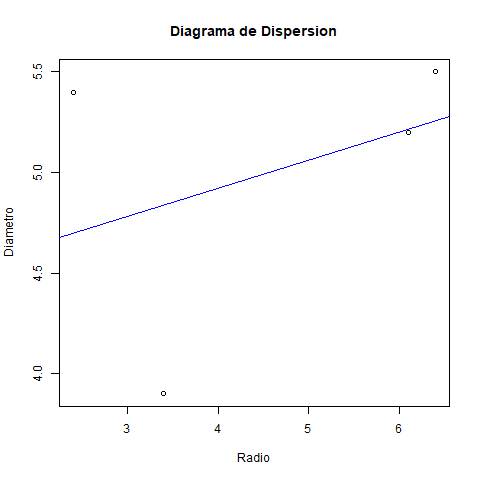
\includegraphics[width=\textwidth]{regPlanetas}

\end{document}
